\documentclass[landscape,archE]{baposter}

\usepackage{times}
\usepackage{calc}
\usepackage{graphicx}
\usepackage{amsmath}
\usepackage{amssymb}
\usepackage{relsize}
\usepackage{multirow}
\usepackage{bm}
\usepackage{subfigure}

\usepackage{graphicx}
\usepackage{multicol}

\usepackage{pgf}
\usepackage{pgfbaselayers}
\pgfdeclarelayer{background}
\pgfdeclarelayer{foreground}
\pgfsetlayers{background,main,foreground}

\usepackage{helvet}
%\usepackage{bookman}
\usepackage{palatino}

\newcommand{\captionfont}{\footnotesize}

\selectcolormodel{cmyk}

\graphicspath{{images/}}

%%%%%%%%%%%%%%%%%%%%%%%%%%%%%%%%%%%%%%%%%%%%%%%%%%%%%%%%%%%%%%%%%%%%%%%%%%%%%%%%
%%%% Some math symbols used in the text
%%%%%%%%%%%%%%%%%%%%%%%%%%%%%%%%%%%%%%%%%%%%%%%%%%%%%%%%%%%%%%%%%%%%%%%%%%%%%%%%
% Format 
\newcommand{\Matrix}[1]{\begin{bmatrix} #1 \end{bmatrix}}
\newcommand{\Vector}[1]{\Matrix{#1}}
\newcommand*{\SET}[1]  {\ensuremath{\mathcal{#1}}}
\newcommand*{\MAT}[1]  {\ensuremath{\mathbf{#1}}}
\newcommand*{\VEC}[1]  {\ensuremath{\bm{#1}}}
\newcommand*{\CONST}[1]{\ensuremath{\mathit{#1}}}
\newcommand*{\norm}[1]{\mathopen\| #1 \mathclose\|}% use instead of $\|x\|$
\newcommand*{\abs}[1]{\mathopen| #1 \mathclose|}% use instead of $\|x\|$
\newcommand*{\absLR}[1]{\left| #1 \right|}% use instead of $\|x\|$

\def\norm#1{\mathopen\| #1 \mathclose\|}% use instead of $\|x\|$
\newcommand{\normLR}[1]{\left\| #1 \right\|}% use instead of $\|x\|$
\def\imagetop#1{\vtop{\null\hbox{#1}}}

%%%%%%%%%%%%%%%%%%%%%%%%%%%%%%%%%%%%%%%%%%%%%%%%%%%%%%%%%%%%%%%%%%%%%%%%%%%%%%%%
% Multicol Settings
%%%%%%%%%%%%%%%%%%%%%%%%%%%%%%%%%%%%%%%%%%%%%%%%%%%%%%%%%%%%%%%%%%%%%%%%%%%%%%%%
\setlength{\columnsep}{0.7em}
\setlength{\columnseprule}{0mm}


%%%%%%%%%%%%%%%%%%%%%%%%%%%%%%%%%%%%%%%%%%%%%%%%%%%%%%%%%%%%%%%%%%%%%%%%%%%%%%%%
% Save space in lists. Use this after the opening of the list
%%%%%%%%%%%%%%%%%%%%%%%%%%%%%%%%%%%%%%%%%%%%%%%%%%%%%%%%%%%%%%%%%%%%%%%%%%%%%%%%
\newcommand{\compresslist}{%
\setlength{\itemsep}{1pt}%
\setlength{\parskip}{0pt}%
\setlength{\parsep}{0pt}%
}


%%%%%%%%%%%%%%%%%%%%%%%%%%%%%%%%%%%%%%%%%%%%%%%%%%%%%%%%%%%%%%%%%%%%%%%%%%%%%%
%%% Begin of Document
%%%%%%%%%%%%%%%%%%%%%%%%%%%%%%%%%%%%%%%%%%%%%%%%%%%%%%%%%%%%%%%%%%%%%%%%%%%%%%

\begin{document}

%%%%%%%%%%%%%%%%%%%%%%%%%%%%%%%%%%%%%%%%%%%%%%%%%%%%%%%%%%%%%%%%%%%%%%%%%%%%%%
%%% Here starts the poster
%%%---------------------------------------------------------------------------
%%% Format it to your taste with the options
%%%%%%%%%%%%%%%%%%%%%%%%%%%%%%%%%%%%%%%%%%%%%%%%%%%%%%%%%%%%%%%%%%%%%%%%%%%%%%
\typeout{Poster Starts}
\background{
  \begin{tikzpicture}[remember picture,overlay]%
    \draw (current page.north west)+(-2em,-0em) node[anchor=north west] {\hspace{-2em}\includegraphics[height=1.1\textheight]{silhouettes_background}};
  \end{tikzpicture}%
}
\definecolor{silver}{cmyk}{0,0,0,0.3}
\definecolor{yellow}{cmyk}{0,0,0.9,0.0}
\definecolor{reddishyellow}{cmyk}{0,0.22,1.0,0.0}
\definecolor{black}{cmyk}{0,0,0.0,1.0}
\definecolor{darkYellow}{cmyk}{0,0,1.0,0.5}
\definecolor{darkSilver}{cmyk}{0,0,0,0.1}
\definecolor{white}{cmyk}{0,0,0,0,}
\definecolor{turquois}{cmyk}{0.3,0,0,0}
\definecolor{purple}{cmyk}{0.8,0.8,0,0}

\definecolor{lightyellow}{cmyk}{0,0,0.3,0.0}
\definecolor{lighteryellow}{cmyk}{0,0,0.1,0.0}
\definecolor{lightestyellow}{cmyk}{0,0,0.05,0.0}

% Define some UCSC colors
\definecolor{ucsc-gold}{RGB}{241,181,33} % Definition from http://www1.ucsc.edu/identity/print-colors.html
\definecolor{ucsc-blue}{RGB}{0,69,140}

\begin{poster}{
  % Show grid to help with alignment
  grid=false,
  % Column spacing
  % Color style
  bgColorOne=white,
  bgColorTwo=white,
  borderColor=black,
  headerColorOne=white,
  headerColorTwo=black,
  headerFontColor=black,
  boxColorOne=white,
  boxColorTwo=white,
  % Format of textbox
  textborder=none,
  % Format of text header
  eyecatcher=false,
  headerborder=none,
  headerheight=0.08\textheight,
  headershape=rectangle,
  headershade=plain,
  headerfont=\Large\textsf, %Sans Serif
%  background=shade-tb,
  columns=3,
  background=plain,
  linewidth=1pt
  }
  % Eye Catcher
  {} % No eye catcher for this poster. If an eye catcher is present, the title is centered between eye-catcher and logo.
  % Title
  {\sf %Sans Serif
  %\bf% Serif
  Autonomy at the Surface: Oceanography through Robotics}
  % Authors
  {\sf %Sans Serif
  % Serif
 Bryant Mairs,
 Prof. Ren Curry, and
 Prof. Gabriel Elkaim \newline
 University of California Santa Cruz \newline
\vspace{-.2in}
\color{ucsc-gold}
\hspace{-.03in}\rule[0.25em]{13.63in}{.09em}
\vspace{-.1in}
  }
  % University logo
  {{\begin{minipage}{16em}
    \hfill
    
\includegraphics[height=12em]{SOE_logo}
  \end{minipage}}
  }

  \tikzstyle{light shaded}=[top color=baposterBGtwo!30!white,bottom color=baposterBGone!30!white,shading=axis,shading angle=30]

  % Width of left inset image
     \newlength{\leftimgwidth}
     \setlength{\leftimgwidth}{0.78em+8.0em}

%%%%%%%%%%%%%%%%%%%%%%%%%%%%%%%%%%%%%%%%%%%%%%%%%%%%%%%%%%%%%%%%%%%%%%%%%%%%%%
%%% Now define the boxes that make up the poster
%%%---------------------------------------------------------------------------
%%% Each box has a name and can be placed absolutely or relatively.
%%% The only inconvenience is that you can only specify a relative position 
%%% towards an already declared box. So if you have a box attached to the 
%%% bottom, one to the top and a third one which should be in between, you 
%%% have to specify the top and bottom boxes before you specify the middle 
%%% box.
%%%%%%%%%%%%%%%%%%%%%%%%%%%%%%%%%%%%%%%%%%%%%%%%%%%%%%%%%%%%%%%%%%%%%%%%%%%%%%
    %
    % A coloured circle useful as a bullet with an adjustably strong filling
    \newcommand{\colouredcircle}[1]{%
      \tikz{\useasboundingbox (-0.2em,-0.32em) rectangle(0.2em,0.32em); \draw[draw=black,fill=baposterBGone!80!black!#1!white,line width=0.03em] (0,0) circle(0.18em);}}

%%%%%%%%%%%%%%%%%%%%%%%%%%%%%%%%%%%%%%%%%%%%%%%%%%%%%%%%%%%%%%%%%%%%%%%%%%%%%%
  \headerbox{ \hspace{7.5em} Objectives}{name=objectives,column=0,row=0}{
%%%%%%%%%%%%%%%%%%%%%%%%%%%%%%%%%%%%%%%%%%%%%%%%%%%%%%%%%%%%%%%%%%%%%%%%%%%%%%
   {}
   {\color{ucsc-blue} \rule{\textwidth}{.1mm}}
   \vspace{0em}

   \begin{tabular}{l l}
   \begin{minipage}{0.6\textwidth}
\textbf{Low-cost oceanography, e.g. surveys of}
\begin{itemize}
  \item the Oxygen Minimum Zone
  \item harmful algal blooms
  \item thin layers
  \item zooplankton
  \item open ocean eddies
\end{itemize}

\textbf{To further research through open-source} as an autonomous research platform. \newline

\textbf{Explore distributed control} across heterogenous vehicle fleets \newline

\textbf{Research carrier capabilities} for rotary-wing aircraft. \newline
   \end{minipage}
   &
   \begin{minipage}{0.4\textwidth}
   \begin{center}
   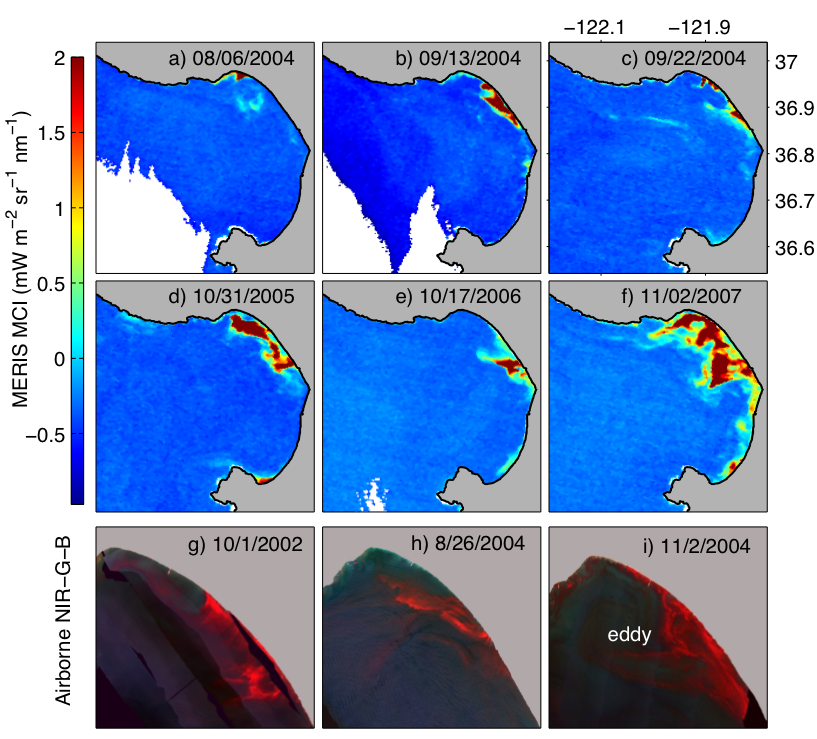
\includegraphics[width=10em]{images/algal_bloom.png} \newline \newline

   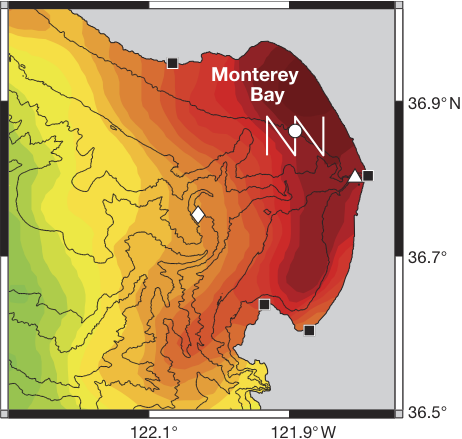
\includegraphics[width=9em]{images/chlorophyll_survey.png}
   \end{center}
   \end{minipage}
   \end{tabular}
 }
 
 %%%%%%%%%%%%%%%%%%%%%%%%%%%%%%%%%%%%%%%%%%%%%%%%%%%%%%%%%%%%%%%%%%%%%%%%%%%%%%
  \headerbox{\hspace{7.9em} Hardware}{name=hardware,column=0,below=objectives,above=bottom}{
%%%%%%%%%%%%%%%%%%%%%%%%%%%%%%%%%%%%%%%%%%%%%%%%%%%%%%%%%%%%%%%%%%%%%%%%%%%%%%
   {}
   {\color{ucsc-blue} \rule{\textwidth}{.1mm}}
   \begin{center}
     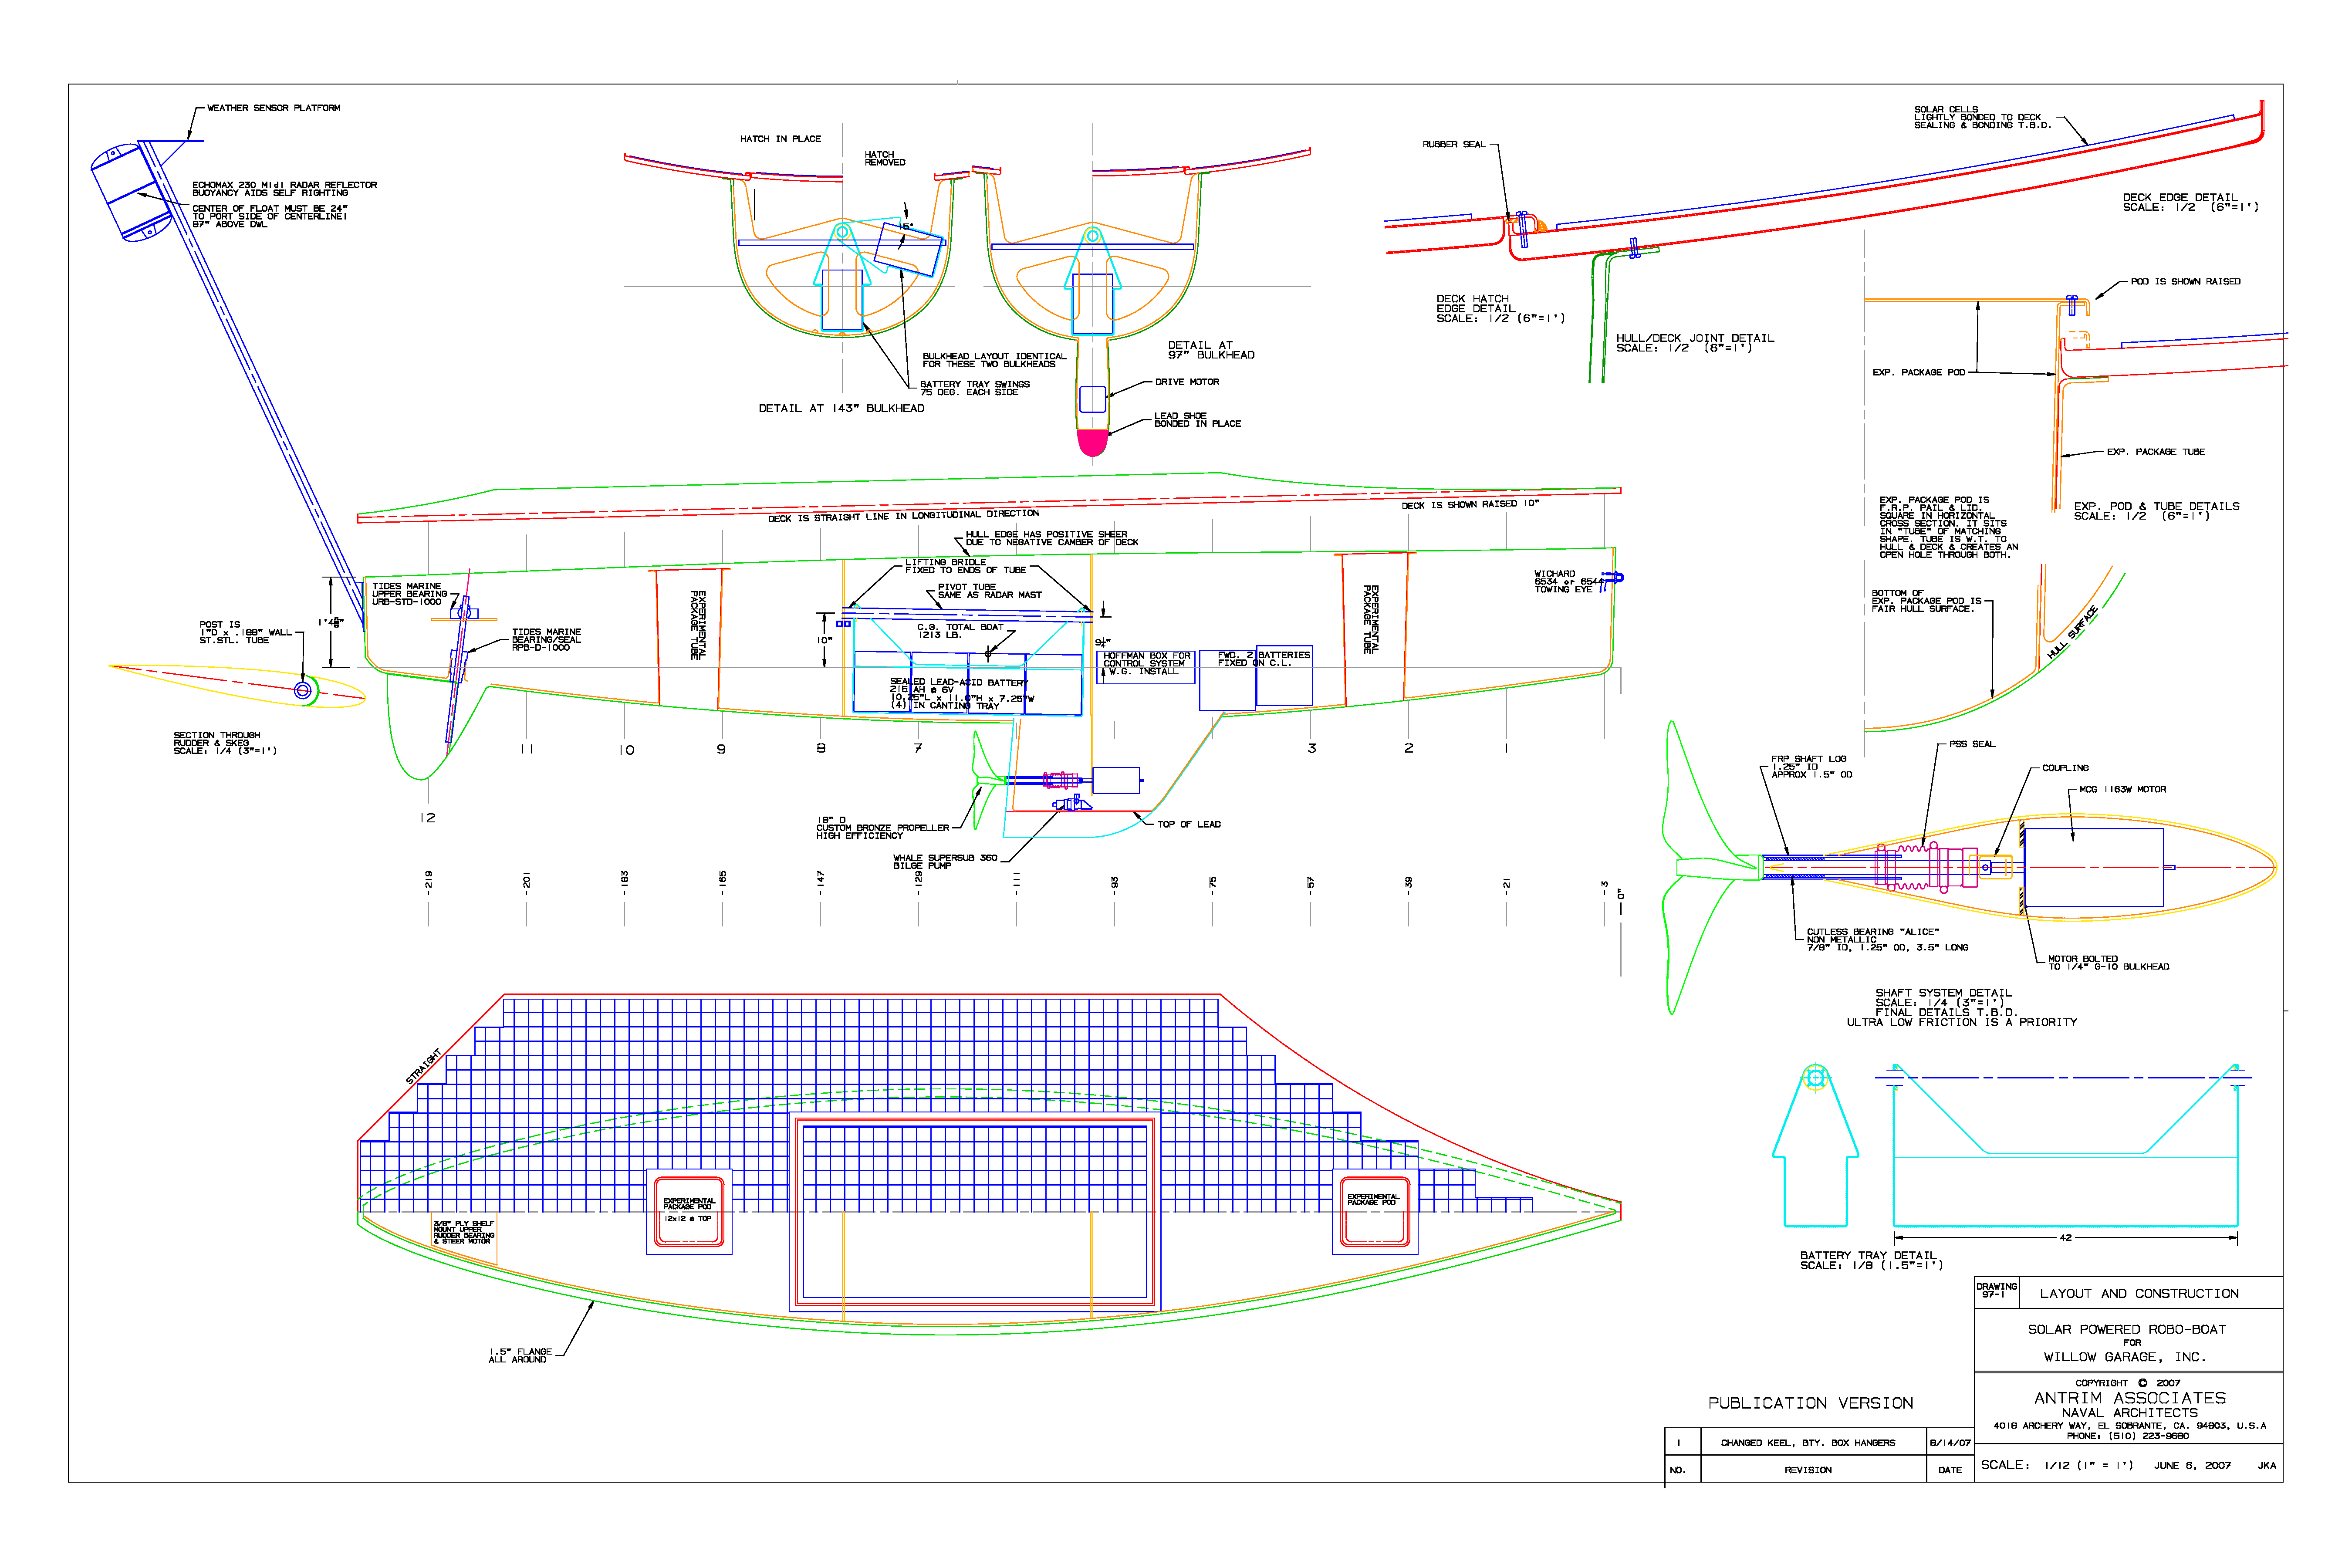
\includegraphics[width=\textwidth,trim=0.9in 0.9in 0.9in 0.9in,clip=true]{Hull.pdf}
   \end{center}

   \vspace{-2em}
   \hspace{-1em}
   \begin{tabular}{p{.4\textwidth} p{.57\textwidth}}
   \begin{center}
      \textbf{Onboard}
   \end{center}

   \begin{itemize}
    \item 3-axis mag, accel, gyro
    \item GlobalSat GPS
    \item Passive radar
    \item Water depth, temp, speed
   \end{itemize}
   &
   \begin{center}
      \textbf{Capabilities}
   \end{center}

   \begin{itemize}
     \item >1kW solar charging power
     \item Mobile ballast for controlling roll
     \item Modular sensor payload
     \item Max cruising speed of 3.7 knots (4.3mph)
     \item Long-range wireless radio
   \end{itemize}
   \end{tabular}
 }
 
 %%%%%%%%%%%%%%%%%%%%%%%%%%%%%%%%%%%%%%%%%%%%%%%%%%%%%%%%%%%%%%%%%%%%%%%%%%%%%%
  \headerbox{\hspace{19.8em} Software}{name=software,column=1,row=0,span=2}{
%%%%%%%%%%%%%%%%%%%%%%%%%%%%%%%%%%%%%%%%%%%%%%%%%%%%%%%%%%%%%%%%%%%%%%%%%%%%%%
   {}
   {\color{ucsc-blue} \rule{\textwidth}{.1mm}}

   \vspace{-0.8em}
   \begin{tabular}{p{.3\textwidth} p{.3\textwidth} p{.3\textwidth}}
   \begin{center}
      \textbf{Software platform}
   \end{center}

   \begin{itemize}
    \item Control algorithms written in MATLAB, Simulink with C drivers provide integration with sensors
    \item Simulation, HIL, and live code from similar code base
    \item Fully open source and retargeteable
   \end{itemize}
   \vspace{2.6em}
   \begin{center}
      \includegraphics[width=17em]{images/navigation_controller.png}
   \end{center}
   &
   \begin{center}
      \textbf{Simulation model}
   \end{center}

   \begin{itemize}
     \item Inverse-bicycle model
     \item Replicates environment down to the actuator level
     \item Augmented with 1\textsuperscript{st} order dynamics determined from live tests
   \end{itemize}
   \vspace{0.5em}
   \begin{center}
      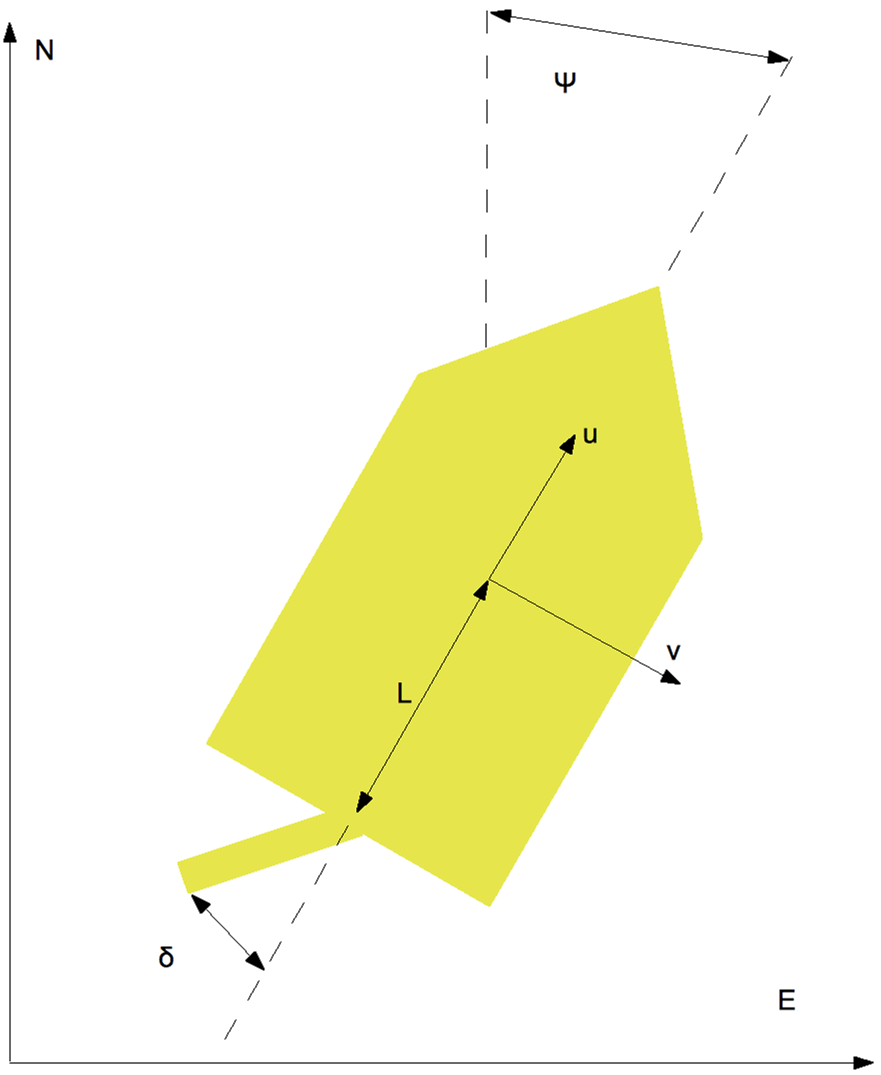
\includegraphics[width=12em]{images/inverse_bicycle.png}
   \end{center}
   &
   \begin{center}
      \textbf{Controller}
   \end{center}

   \begin{itemize}
     \item Utilizes L2+ Guidance, a robust derivative of L1 control
     \item Look-ahead vector (L$_\text{1}$) determines intercept point along desired line trajectory
     \item Crosstrack and velocity PID loops provide path control
   \end{itemize}

   \vspace{0em} % Necessary
   \begin{center}
      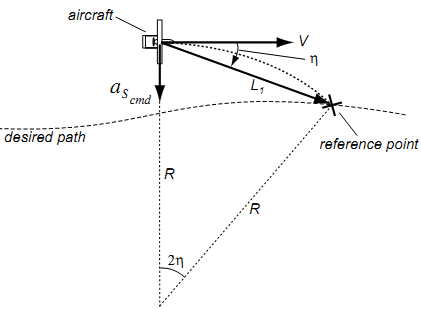
\includegraphics[width=17em]{images/L1-control.png}
   \end{center}
   \end{tabular}

   \vspace{-2em}
 }
 
 %%%%%%%%%%%%%%%%%%%%%%%%%%%%%%%%%%%%%%%%%%%%%%%%%%%%%%%%%%%%%%%%%%%%%%%%%%%%%%
  \headerbox{\hspace{7.9em} Results}{name=future,column=1,row=1,above=bottom, below=software}{
%%%%%%%%%%%%%%%%%%%%%%%%%%%%%%%%%%%%%%%%%%%%%%%%%%%%%%%%%%%%%%%%%%%%%%%%%%%%%%
   {}
   {\color{ucsc-blue} \rule{\textwidth}{.1mm}}
   \vspace{0em}

   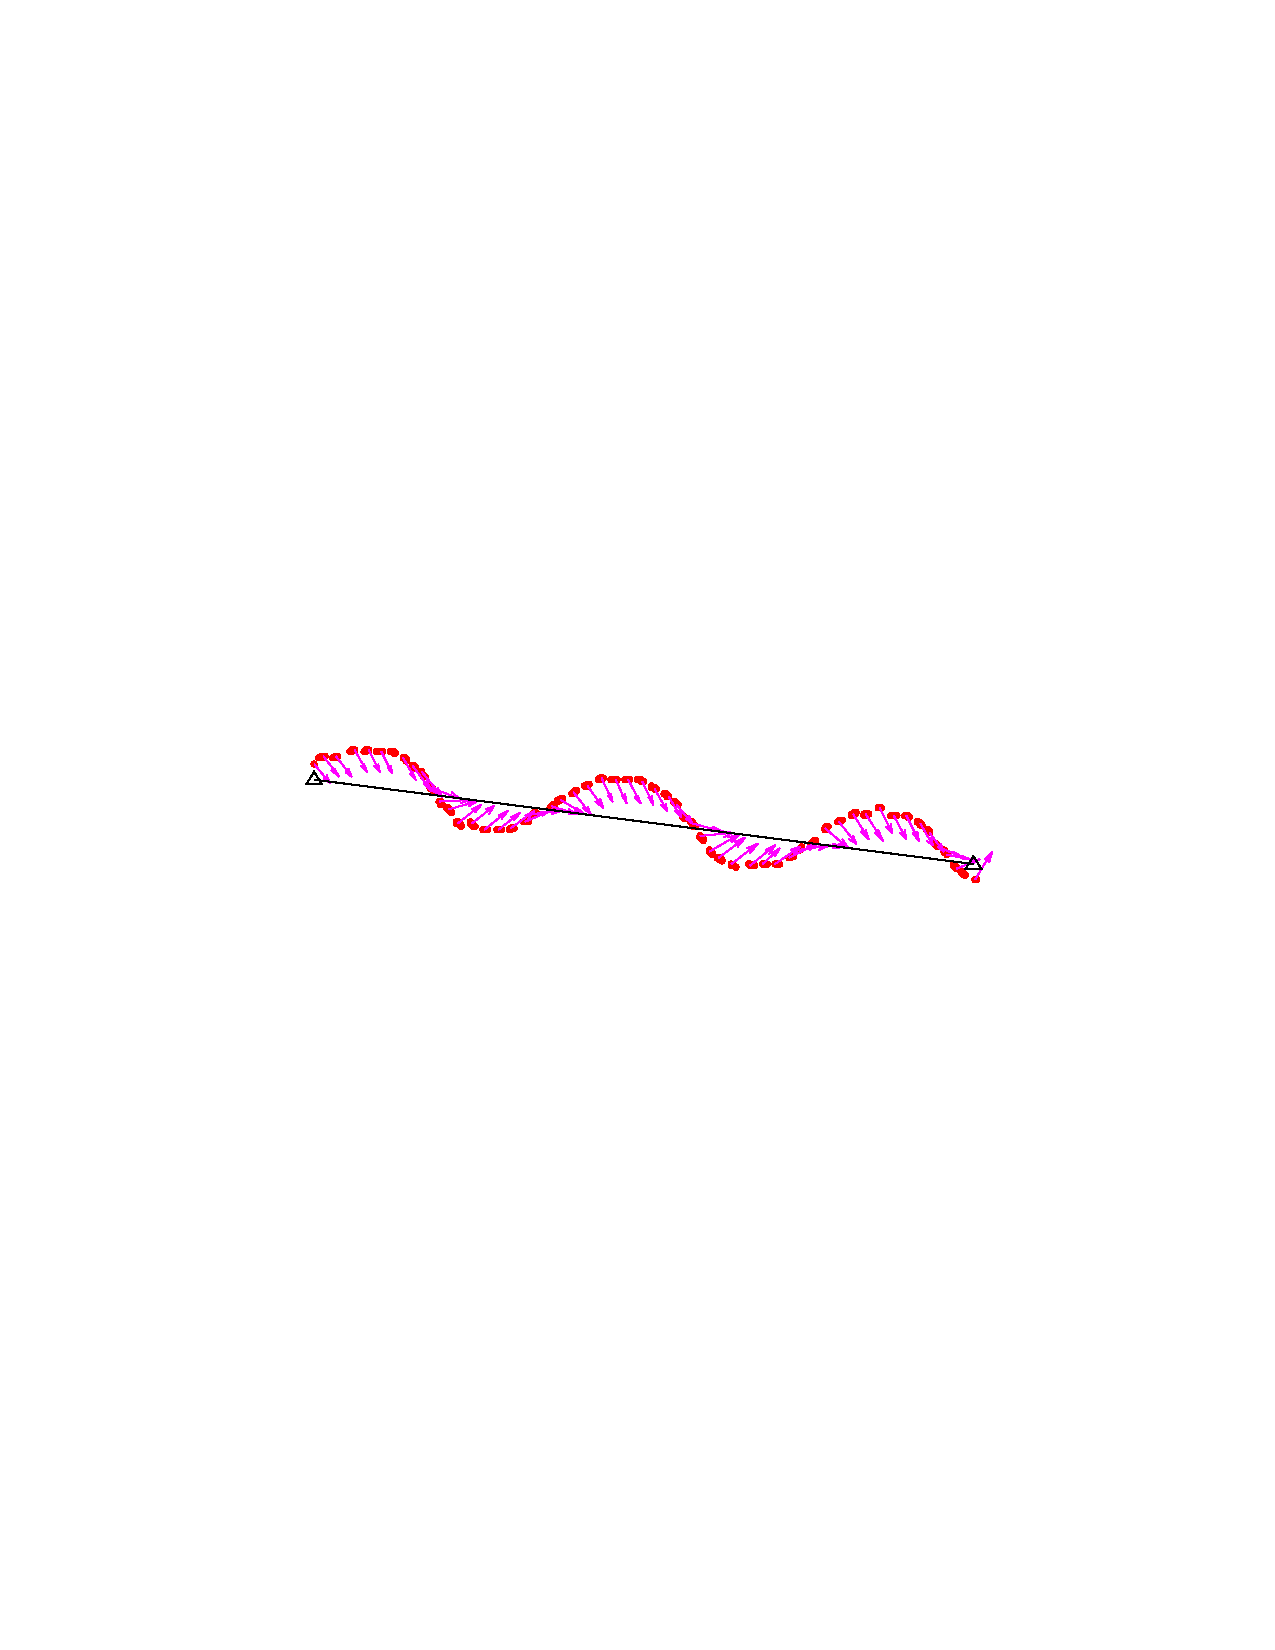
\includegraphics[width=\textwidth,trim=2in 5.1in 1.8in 4.95in,clip=true]{images/figure1.pdf}
   \begin{center}
      \textbf{First autonomous line-following test} \\
      \small{Purple: desired heading} \\
      \small{Black: desired path} \\
   \end{center}

   \vspace{1em}
   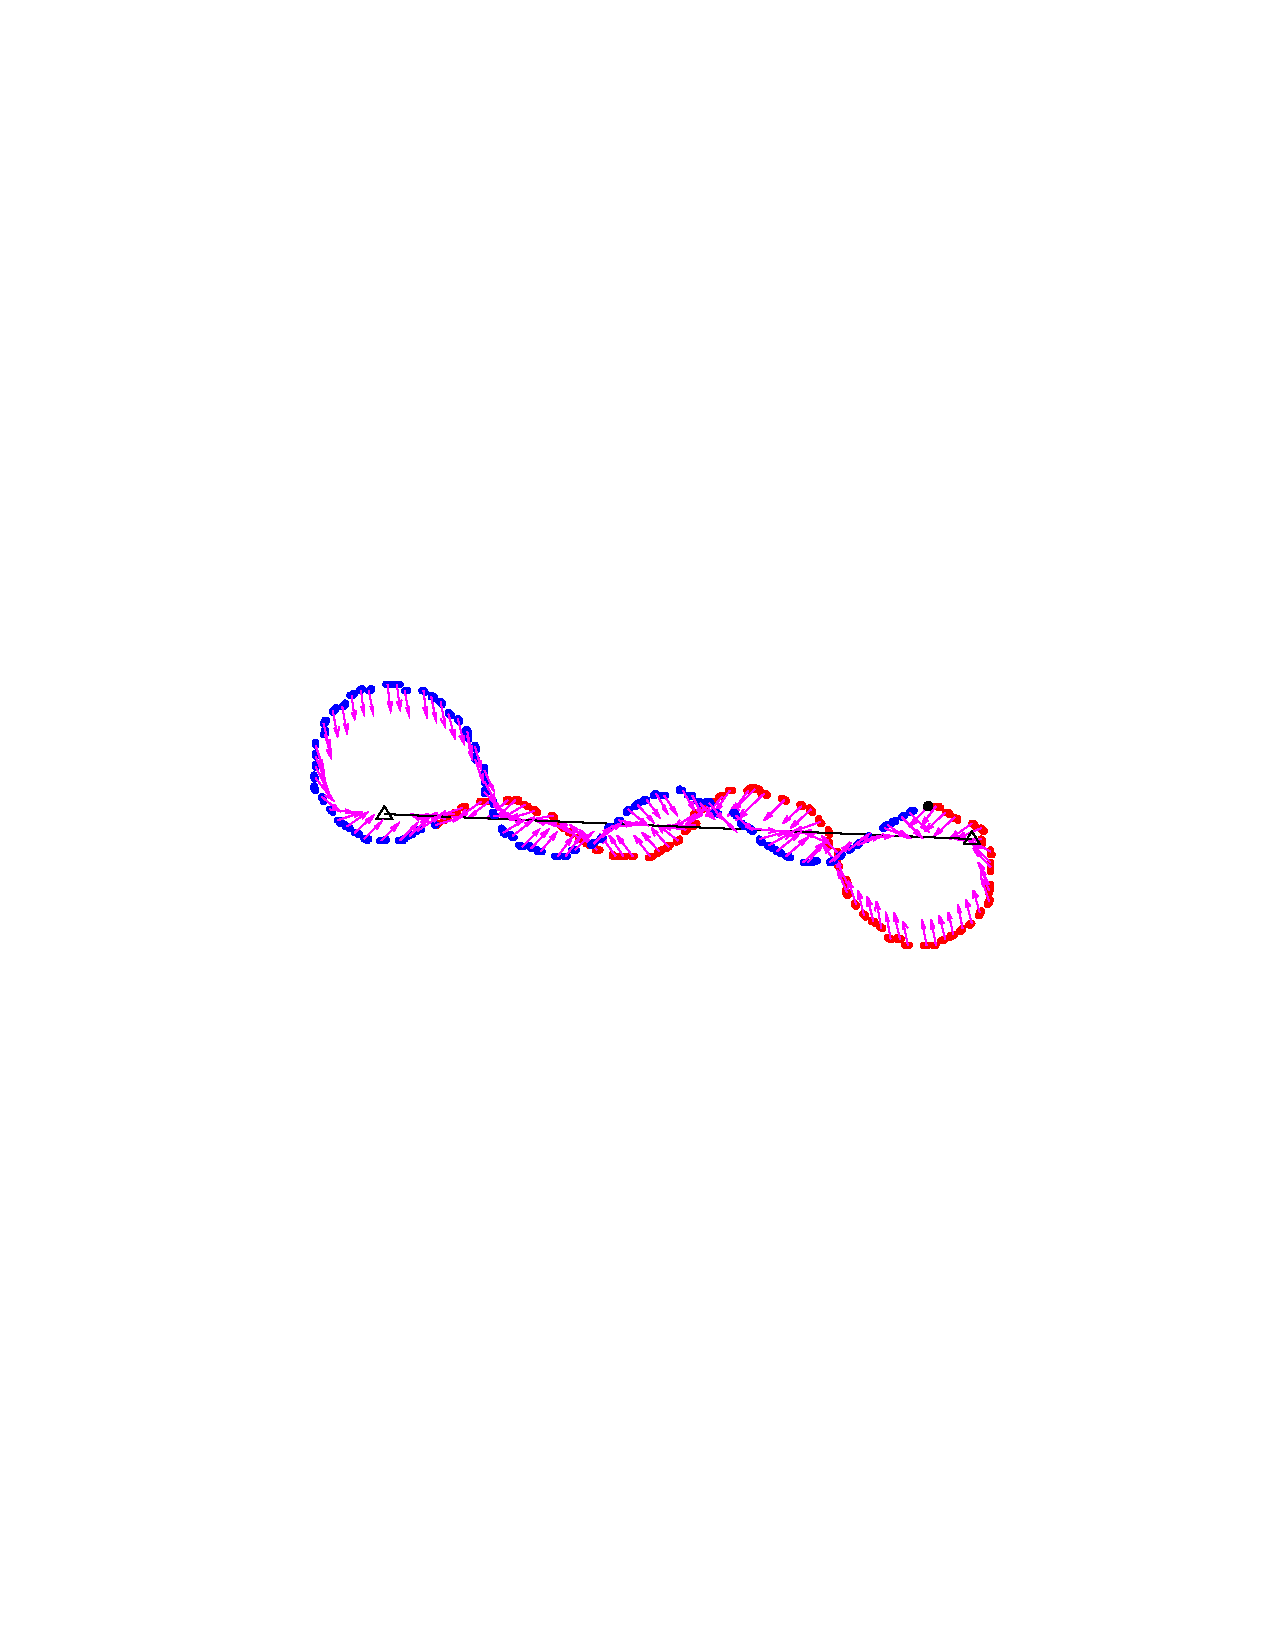
\includegraphics[width=\textwidth,trim=2in 4.65in 1.8in 4.5in,clip=true]{images/figure2.pdf}
   \begin{center}
      \textbf{Test of autonomous waypoint switching} \\
      \small{Red: westward trajectory (initial point in black), Blue: eastward trajectory} \\
      \small{Purple: desired heading, Black: desired path} \\
   \end{center}
 }
 
 %%%%%%%%%%%%%%%%%%%%%%%%%%%%%%%%%%%%%%%%%%%%%%%%%%%%%%%%%%%%%%%%%%%%%%%%%%%%%%
  \headerbox{\hspace{7.9em} Current Focus}{name=future,column=2,row=1,above=bottom, below=software}{
%%%%%%%%%%%%%%%%%%%%%%%%%%%%%%%%%%%%%%%%%%%%%%%%%%%%%%%%%%%%%%%%%%%%%%%%%%%%%%
   {}
   {\color{ucsc-blue} \rule{\textwidth}{.1mm}}
   \begin{itemize}
      \item Improved vehicle model
      \item Complimentary filters for estimation of slow sensors (GPS)
      \item Integration of intertial measurement unit (IMU)
      \item Bi-directional remote command interface through the use of \newline the open-source QGroundControl project already in use  by \newline SLUGS
   \end{itemize}
   \vspace{1em}
   \begin{center}
       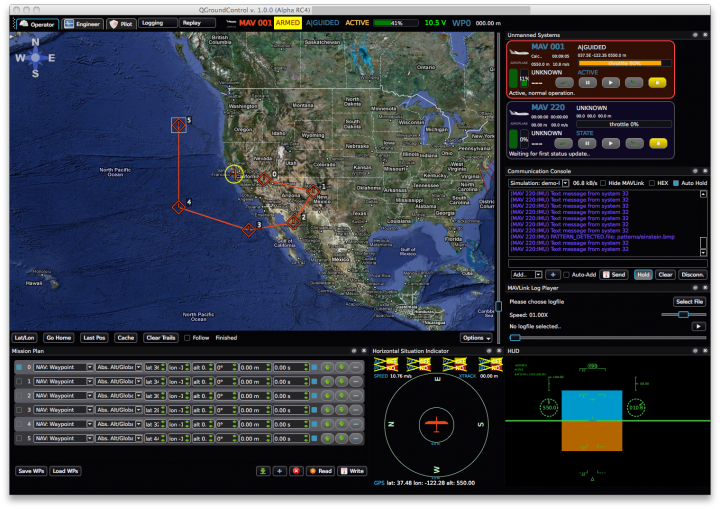
\includegraphics[width=0.7\textwidth]{images/qgroundcontrol_operator_2dmap.png}
   \end{center}
 }

\end{poster}
\end{document}
